\documentclass[11pt,a4paper]{article}
\usepackage{url}
\usepackage{graphicx}
\usepackage{amsmath}
\usepackage{amsfonts}
\usepackage{amssymb}
\usepackage{subcaption}

\begin{document}

\begin{titlepage}
	\centering % Centre everything on the title page
	\vspace*{\baselineskip} 
	
	\rule{\textwidth}{1.6pt}\vspace*{-\baselineskip}\vspace*{2pt} % Thick horizontal rule
	\rule{\textwidth}{0.4pt} % Thin horizontal rule
	
	\vspace{0.75\baselineskip}
	{\scshape\LARGE Extreme Rainfall Prediction\\ In\\ India \\} 
	\vspace{0.75\baselineskip} 
	
	\rule{\textwidth}{0.4pt}\vspace*{-\baselineskip}\vspace{3.2pt}
	\rule{\textwidth}{1.6pt} 
	
	\vspace{2\baselineskip}
	{\scshape CS685 Project Report\\}
	\vspace*{3\baselineskip}
	{\scshape Group 7}
	
	\vspace{0.5\baselineskip}
	
	{\large  Debanjan Chatterjee - 20111016 (debanjan20@iitk.ac.in)\\P J Leo Evenss - 20111038 (leoevenss20@iitk.ac.in)\\ Shilpa Chatterjee - 20111057 (shilpa20@iitk.ac.in) \\Shruti Sharma - 20111061 (shruti20@iitk.ac.in)  \\ Bopanna Tej Kiran - 20111070(tejkiranb20@iitk.ac.in)}
	
	\vspace{2.8\baselineskip}
	\textit{Indian Institute of Technology, \\ Kanpur} 	
	\vspace{2.8\baselineskip}
	
	2020
\end{titlepage}
\section{Abstract}
Prediction of extreme rainfall is an important problem in the field of meteorology as it has an enormous impact on the life of people and a nation's economy. Every year people across the globe suffer from severe consequences of heavy rainfall like flood, spread of diseases,loss of life and belongings etc.\\

In this project we tried to predict extreme rainfall events 24 h to 48 h before the occurrence of the event using the previous climatic parameters. We tested various machine learning models on districts covering the entire Indian subcontinent. However, due to the problem of class imbalance, the model predicted several false positives and false negatives during classification. We tried to solve this issue through SMOTE.

\section{Literature}
Importance of Summer Monsoons to country's economy and its variability has motivated scientists to study these variations. They rigorously examine the weather patterns and deduce studies to prevent adverse effects of flood situations.\\
The 22 features considered in this study have been found to be important factors influencing rainfall.

 \section{Problem Statement}
The available methods for heavy rainfall prediction are able to predict only 6 h prior to the event. We have tried to address the problem of predicting the occurrence of extreme rainfall events across regions during the summer monsoon months of June-September. The prediction is done based on the weather conditions over the region and it’s surroundings in the past 48 h to 24 h. This will ensure that least damage is caused by heavy rainfall events.
 \\
 
 For this purpose, we have used historical data of important weather variables that affect rainfall and trained our model. It is then tested with a new set of feature values to give a binary prediction about the extreme rainfall occurrence in the next 24–48 hrs.
 
\section{Introduction}
The science of climatic extremes is important and critical in terms of modeling, socio-economic impacts, damages, and adaptation.Though there has been significant research advancements in the field of meteorology, there are still notable number of extreme events resulting in huge human and economic losses. One such event was Assam flood that started in May 2020 due to heavy rainfall affecting 30,000 and destroying crops across 5 districts.\\

As of October 2020, according to \url{https://en.wikipedia.org/wiki/2020_Assam_floods}, the floods affected over five million people, claiming the lives of 123 people, with an additional 26 deaths due to landslides, 5474 villages were affected and over one hundred and fifty thousand people found refuge in relief camps. This highlights the importance of early prediction of extreme rainfall.

\section{Motivation} 
Heavy rainfall can occur due to some anomalous weather features prevalent in areas far away from the region of interest. We have therefore used the weather features over the entire Indian subcontinent. This will help in capturing the non-homogeneity in land-sea interaction, weather system and topography, over entire India, which affects rainfall in all parts of the country. 


\section{Dataset}
We have obtained the weather parameters for the entire Indian subcontinent from National Centers for Environmental Prediction/National Center for Atmospheric Research (NCEP/NCAR) reanalysis dataset. The latitude ranges from 5 degrees to 40 degrees north and longitude ranges from 65 degrees to 100 degrees east. In particular we have used daily data of weather parameters at surface and multiple levels from \url{https://psl.noaa.gov/data/gridded/data.ncep.reanalysis.surface.html }.\\

The NCEP/NCAR reanalysis data has a spatial grid resolution of 2.5\textdegree \  * 2.5\textdegree. The region is divided into 225 grids. So there are a total of 22*225 = 4950 variables available for each day since daily data is taken. For 48 h as well as 24 h prior prediction, the variables are increased to 4950*2 = 9900. \\

The surface level parameters are air temperature, mean sea level pressure, precipitable water, relative humidity, vertical wind velocity (omega), U-wind and V-wind. For multiple levels we have considered weather parameters at 850-, 600- and 400-hPa levels.The 850-,600-, 400-hPa level variables are air temperature, vertical wind velocity (omega),
 relative humidity, U-wind and V-wind. The surface and multiple level parameters sum up to 22 in total.
\medskip

The weather parameters have been collected for the summer monsoon months in India i.e. June - September for the years 1997–2016.\\

The rainfall data is collected for the same time period from India Meteorological Department (IMD) (\url{http://imdpune.gov.in/Clim_Pred_LRF_New/Grided_Data_Download.html})

\section{Methodology}
The validity of any statistical analysis depends on the quality of the data used in the analysis. Subdivisions are distributed fairly uniformly over the country, so  districts from each subdivision were selected to form the network. A total of 9900 features were used. 

There are 36 meteorological subdivisions of India.
\begin{figure}[!h]
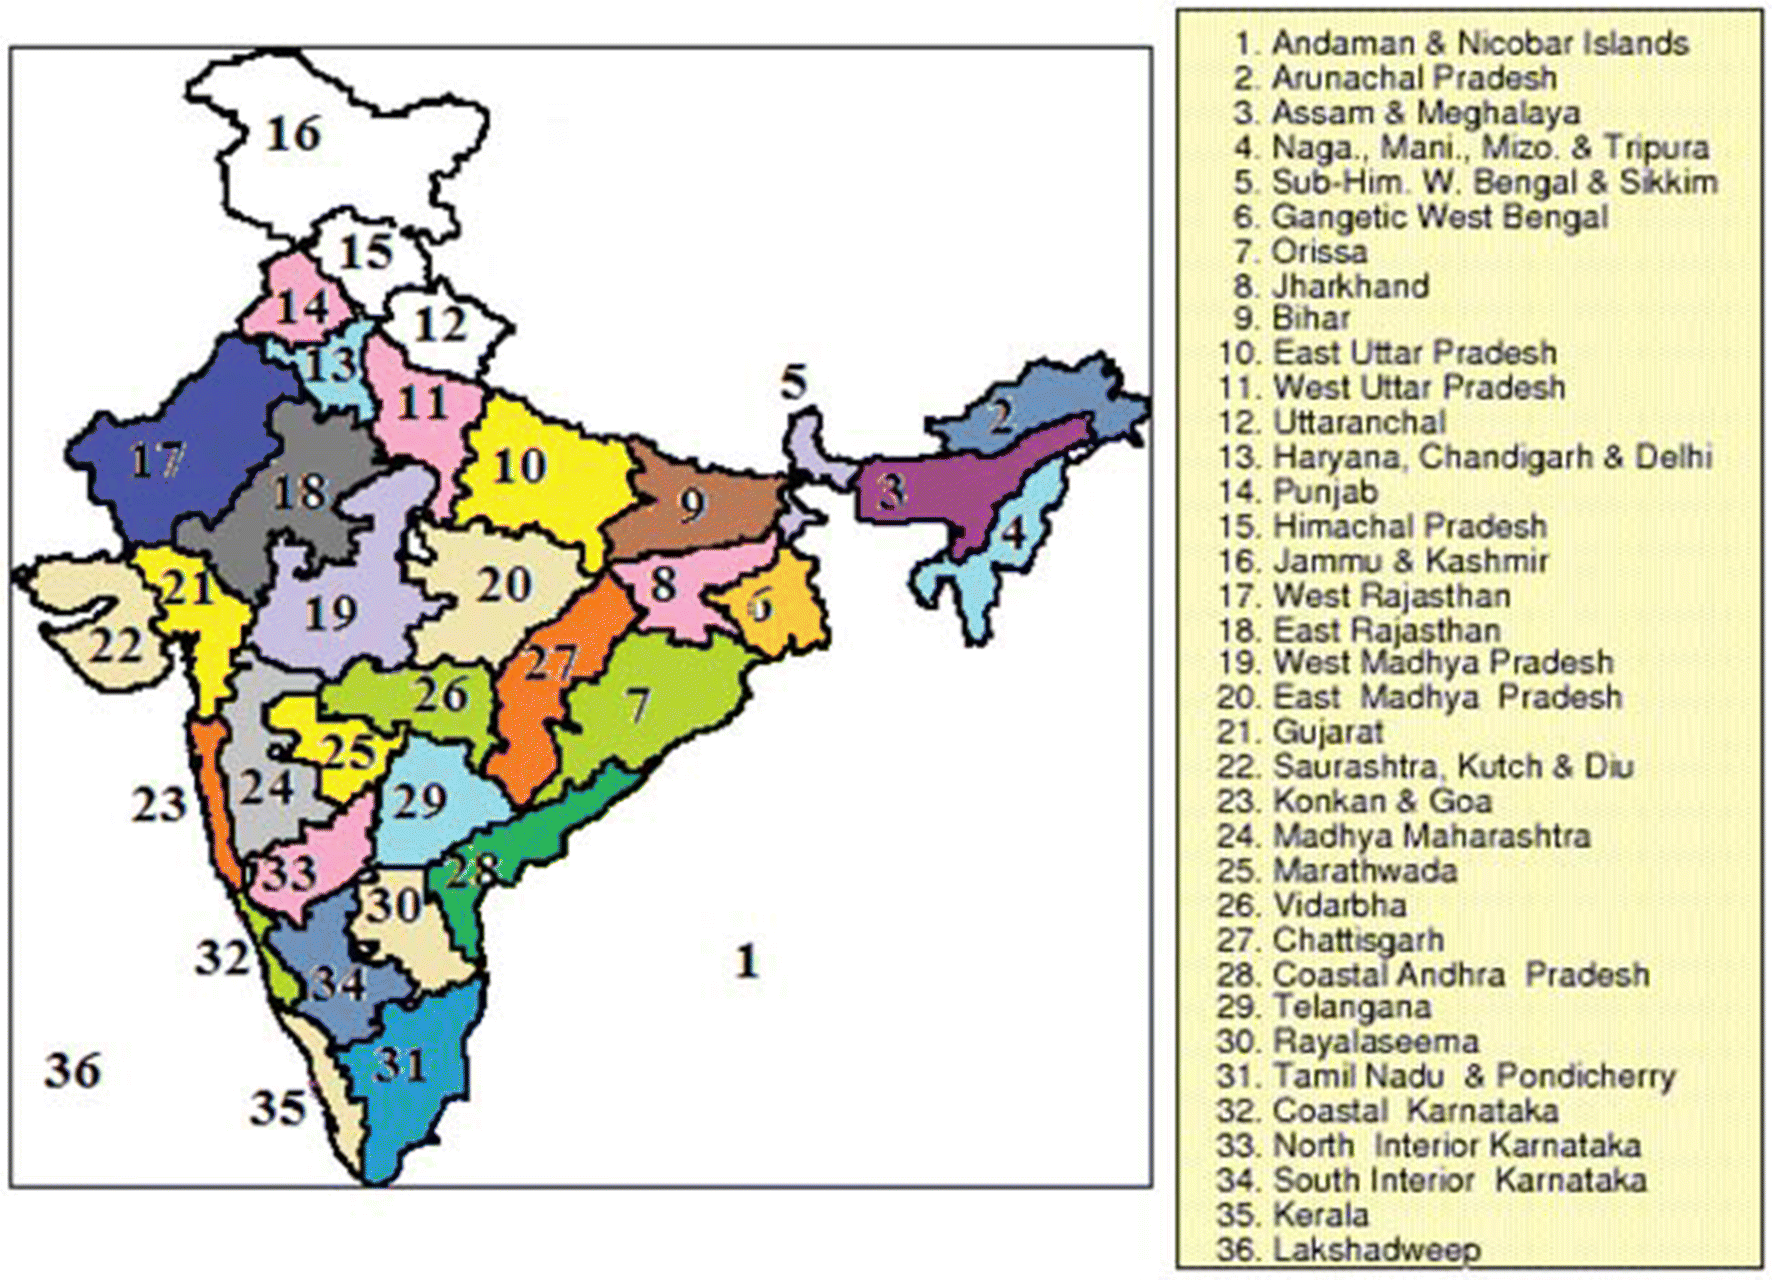
\includegraphics[scale=0.2]{Fig1.png}
\caption{}
\end{figure}
\footnote{\small Image Source: Meteorological Subdivision - OGD Platform India}

Missing values are flagged with -9.96921e+36f. \\

Threshold to determine extreme rainfall at a region = \textit{Region's mean rainfall + Region's standard deviation from mean rainfall.}

\medskip

We started with a set of 7 features namely air temperature, mean sea level pressure, precipitable water, relative humidity, vertical wind velocity (omega), U-wind and V-wind at the surface level.  The Indian subcontinent was divided into equi-sized 225 grids and the daily data was prepared from these resulting in 225 * 7 =1575 features per day. The model trained with these features 
resulting in precision = 0.60 and recall = 0.16. \\

The features were then scaled up considering the different air pressure levels of  850-, 600- and 400-hPa and then dataset amounted to 22 feature attributes , thus 225 * 22=4950 per day and 4950 * 2=9900 for 2 consecutive days.

\medskip

\begin{center}
\textbf{Feature Reduction}
\end{center}

\textbf{Method 1 : Auto-encoder}- Such huge set of features if used for training a machine learning model may lead to overfitting. Therefore, we need a feature reduction technique. In this study, we want to learn the weather attributes which are mainly real-numbered and thus have chosen an auto-encoder architecture of deep learning for the purpose\cite{AE}. A simple auto-encoder is an unsupervised one layered neural network where the input X = $x_1, x_2, ..., x_n$ is a n dimensional feature vector. The output is
given by (f is a non-linear transformation):
\begin{align*}
h_{W,b}(X) = f(W^TX) = f(\sum_{i=1}^N W_ix_i + b)
\end{align*}
The hidden layer gets to learn a compressed representation of the input, such that the original input can be regenerated from it. The loss function is minimized through gradient descent. \\

\textbf{Architecture} -
\begin{itemize}
\item An input layer, (bias b = 9900)
\item 2 hidden layers (initial units = 2500, bias = 2500),
\item An output layer (bias = 9900)
\item Activation function - Sigmoid
\item Optimizer - Adagrad
\item Learning rate - 0.1
\item Batch size - 100
\item Cost function - MSE
\end{itemize}
The first two layers make up an encoder while next two are the decoder. The shapes of input and output layers are same. The number of units in each layer has been set by trial and error. We multiply the output of input layer with a weight matrix and add biases, then take it through the sigmoid activation function and repeat the same for subsequent layers. The weights and biases get updated continuously as we train the model.\\
The size of encoded features comes out to be 2500 from initial 9900. This reduced, compact feature set can be used as input features for further processing. 

\medskip

\textbf{Method 2 : Kernel PCA} - RBF kernel was used. The feature set reduced to 2369 from 9900. However, it was experimentally found that the performance of autoencoder was superior to Kernel PCA.

\medskip


\begin{center}
\textbf{Feature Scaling} 
\end{center}
Since the range of values of raw data varies widely, objective functions will not work properly without normalization. For example, many classifiers calculate the distance between two points by the Euclidean distance. If one of the features has a broad range of values, the distance will be governed by this particular feature. Therefore, range of all the features should be normalized so that each feature contributes approximately proportionately to the final distance.

Another reason why feature scaling is applied is that gradient descent converges much faster with feature scaling than without it. And since, we used XGBoost which inherently uses gradient descent approaches we standardised our dataset using StandardScaler() from sklearn.

\medskip

\begin{center}
\textbf{Class Imbalance }
\end{center}
To effectively deal with the class imbalance problem in our biased dataset and to get the best performance, oversampling of the minority class has been tackled using SMOTE (Synthetic Minority Over-sampling TEchnique)\cite{SMOTE} since features are continuous and we are solving a classification problem. In this new examples are synthesized from the existing examples. 

\begin{figure}[!h]
\begin{subfigure}{.5\textwidth}
\centering
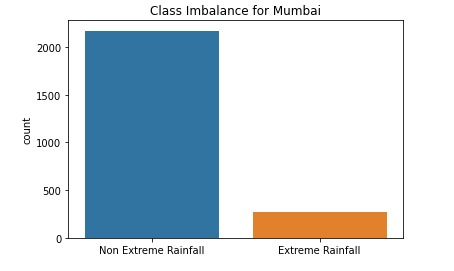
\includegraphics[width=\linewidth]{Fig3.jpeg}
\caption{Skewness in Mumbai Rainfall data}
\end{subfigure}%
\begin{subfigure}{.5\textwidth}
\centering
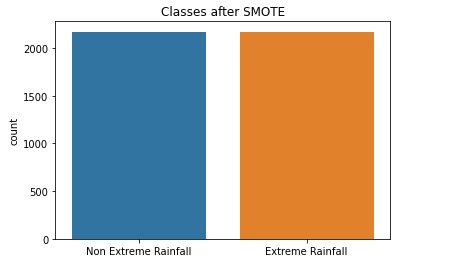
\includegraphics[width=\linewidth]{fig4.jpeg}
\caption{After applying SMOTE}
\end{subfigure}
\end{figure}

SMOTE works by utilizing a k-nearest neighbor algorithm to create synthetic data. The procedure is repeated enough times until the minority class has the same proportion as the majority class.

\section{Results}
\subsection{\textbf{Auto-encoder + SMOTE + XGB (24 h, Mumbai)}} - High recall after dealing with all kinds of problems the data had originally, since Mumbai is one such city that receives heavy rainfall during summer monsoon months.
\begin{figure}[!htp]
\begin{subfigure}{.5\textwidth}
\centering
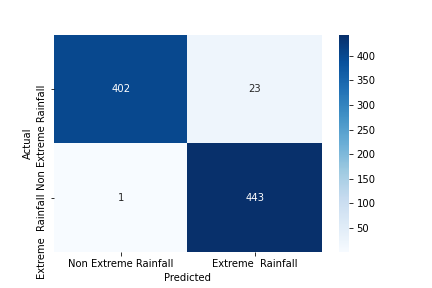
\includegraphics[width=\linewidth]{y_mumbai.png}
\caption{Confusion Matrix}
\end{subfigure}%
\begin{subfigure}{.5\textwidth}
\centering
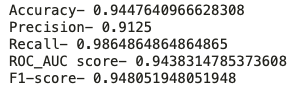
\includegraphics[width=.8\linewidth]{res_mumbai.png}
\caption{Metrics}
\end{subfigure}
\end{figure}

\medskip

\subsection{\textbf{Auto-encoder + XGB (48 h, Mumbai)}} - Low recall because of class-imbalance. Also 24 h prediction performs better than 48 h.
\begin{figure}[!h]
\centering
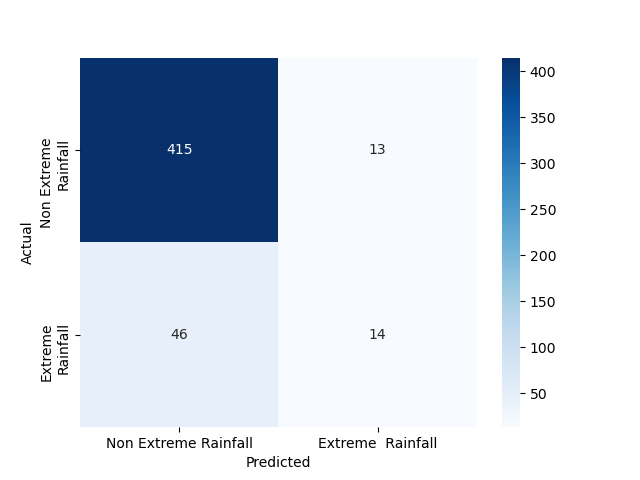
\includegraphics[width=.4\linewidth]{mumbai.png}
\caption{Confusion Matrix}
\end{figure}

\textbf{\small Other Metrics} \begin{itemize}
\item Accuracy - 0.87
\item Precision - 0.51
\item Recall - 0.23
\item F1-score - 0.32
\end{itemize}

\medskip

\subsection{\textbf{XGB (24 h, Mumbai)}} - Low recall because no preprocessing done to balance the dataset.
\begin{figure}[!ht]
\begin{subfigure}{.5\textwidth}
\centering
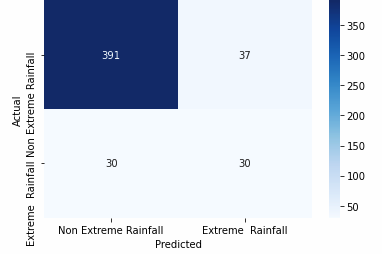
\includegraphics[width=\linewidth]{xgb.png}
\caption{Confusion Matrix (XGB)}
\end{subfigure}%
\begin{subfigure}{.5\textwidth}
\centering
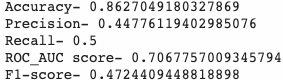
\includegraphics[width=.8\linewidth]{xgb_metrics.png}
\caption{Metrics}
\end{subfigure}
\end{figure}

\medskip

\subsection{\textbf{SVM}} - RBF kernel used. 
\begin{figure}[!ht]
\begin{subfigure}{.5\textwidth}
\centering
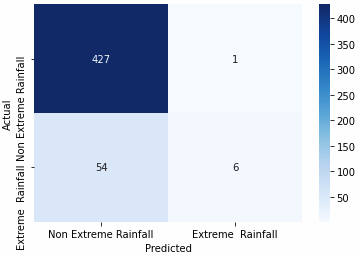
\includegraphics[width=\linewidth]{svm_mumbai.png}
\caption{Confusion Matrix (SVM)}
\end{subfigure}%
\begin{subfigure}{.5\textwidth}
\centering
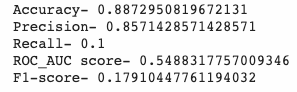
\includegraphics[width=.8\linewidth]{svm_metrics.png}
\caption{Metrics}
\end{subfigure}
\end{figure}
 
 \medskip
 
 \section{Discussion}
 In this work we have explored techniques to learn and represent weather features and use them to predict extreme rainfall events. This model works better because we include all the features and try to understand underlying patterns and dependencies unlike other approaches which rely on selective feature reduction.\\

\begin{itemize}
\item For the country as a whole, the summer monsoon rainfall do not show any significant trend. However, there are large variations at the regional scale.
\item Increasing parameters from 7 to 22 improved the quality of results to a great extent.
\item 24 h prediction gave better results on average than 48 h.
\item SMOTE gave excellent results.
\item For model without SMOTE, even though a cost-sensitive model was used, the performance of model degraded, especially for cities with low percentage of extreme rainfall days, and thus made the dataset more skewed.
\end{itemize}

 \section{Future Direction}
 Here we have solved only a classification problem where we are only able to predict whether there will be heavy rainfall or not. In future we would also like to predict the amount of rainfall as well with the improved methods.

\begin{thebibliography}{9}
\bibitem{SMOTE} Chawla, N.V., Bowyer, K.W., Hall, L.O., Kegelmeyer, W.P.: SMOTE: synthetic minority over-sampling technique. J. Artif. Intell.
\bibitem{} Goswami, B.N., Venugopal, V., Sengupta, D., Madhusoodanan, M., Xavier, P.K.: Increasing trend of extreme rain events over India in a warming environment.
\bibitem{AE} Hinton, G.E., Salakhutdinov, R.R.: Reducing the dimensionality of data with neural networks.
\bibitem{} Sulagna Gope, Sudeshna Sarkar, Pabitra Mitra, and Subimal Ghosh : Early Prediction of Extreme Rainfall Events: A Deep Learning Approach
\end{thebibliography}
\end{document}
